Textual description of trade policy that 
led to the dispute is formally called as
\textit{Factual Aspect} in WTO DSB. 
Since Panels
always provide a factual aspect\footnote{
    It's worth noting that Appellate Body doesn't provide any factual aspect because they use the factual aspect provided by the Panel.
}
that summarizes the content of the dispute
in the panel report (Figure \ref{fig:panel-report-toc}),
this paper wrote a program that can 
automatically search and collect 
the panel reports from the WTO official doucment website\footnote{
    \url{http://docs.wto.org}
}.
Then I wrote another program that locates the start 
and end page of the factual asepct using the information inside the 
table of contents of the report (Figure \ref{fig:panel-report-toc}).
By using this location, I excerpted factual aspect\footnote{
    \hyperref[sub:factual-aspect-example]{Appendix A.1} shows an
    example of excerpted factual aspect from the panel report for \textit{US - Offset (Byrd Amendment)}.    
}
from each panel report listed in Figure \ref{fig:ds-cases-used}. 
Total number of panel reports listed in Figure \ref{fig:ds-cases-used} is 143.

\subsubsection{Joint Adjudication \& Early Settlement}

The number 143 seems small compared to the total number of cases requested to WTO DSB, 596\footnote
{
    As of November 1st, 2020.
}. This is because, first, panel handles different cases requested by different members
for the same trade policy of a member together. For example, in \textit{US - Offset (Byrd Amendment)}, panel merged DS217\footnote{
    DS refers to Dispute Settelement. DS is a officially used prefix that notates the case number in WTO DSB.
} and DS234 together because both were asking inconsistency to the WTO agreements for the same government measure of the United States (Figure \ref{fig:linked-cases}). This paper selects the smallest case number as a representatitve case number for the collected panel reports. For example, in case DS217 and DS234 shares the same panel report, we choose DS217 as a representatitve number for the shared panel report as shown in Figure \ref{fig:ds-cases-used} where DS217 is included but not DS234.

Secondly, members sometimes find \textit{mutually agreeable solution} before the panel expresses its judicial opinion. Then panel stops there and does not publish any panel report, thus no factual aspect is available. This paper omitted this kind of early settled cases from the data collection.

 
% \subsubsection{Judicial Economy \& Early Settlement}

\begin{figure}[h]
    \begin{quote}
        DS 2, 
        18, 
        22, 
        31, 
        34, 
        46, 
        56, 
        58, 
        60, 
        62, 
        67, 
        68, 
        69, 
        75, 
        76, 
        87, 
        90, 
        98, 
        103, 
        108, 
        121, 
        122, 
        135, 
        136, 
        139, 
        141, 
        146, 
        152, 
        155, 
        161, 
        162, 
        165, 
        166, 
        174, 
        175, 
        177, 
        184, 
        202, 
        207, 
        212, 
        217, 
        219, 
        221, 
        231, 
        234, 
        238, 
        244, 
        245, 
        246, 
        248, 
        257, 
        264, 
        265, 
        266, 
        267, 
        268, 
        269, 
        276, 
        282, 
        283, 
        286, 
        290, 
        294, 
        295, 
        296, 
        301, 
        302, 
        308, 
        312, 
        315, 
        316, 
        320, 
        321, 
        322, 
        332, 
        336, 
        339, 
        343, 
        344, 
        345, 
        350, 
        353, 
        360, 
        363, 
        366, 
        371, 
        379, 
        381, 
        384, 
        392, 
        394, 
        396, 
        397, 
        399, 
        400, 
        406, 
        412, 
        414, 
        415, 
        422, 
        425, 
        427, 
        429, 
        430, 
        431, 
        435, 
        436, 
        437, 
        440, 
        442, 
        447, 
        449, 
        453, 
        454, 
        456, 
        457, 
        461, 
        464, 
        468, 
        471, 
        472, 
        473, 
        475, 
        476, 
        477, 
        479, 
        480, 
        482, 
        483, 
        484, 
        485, 
        486, 
        488, 
        490, 
        492, 
        493, 
        495, 
        499, 
        504, 
        505, 
        513, 
        518, 
        523
    \end{quote}
    \caption{
        List of case numbers of collected panel reports. ``DS + number'' uniquely identifies each dispute. For example, DS 523 refers to \textit{US — Pipe and Tube Products (Turkey)} where United States was challenged by Turkey for its possibly inconsistent anti-dumping measure.
        % where Turkey claimed claimed possible illegal trade policy of United States on pipe ane tube products from Turk. 
    }
    \label{fig:ds-cases-used}
\end{figure}

\begin{figure}[h]
    \centering
    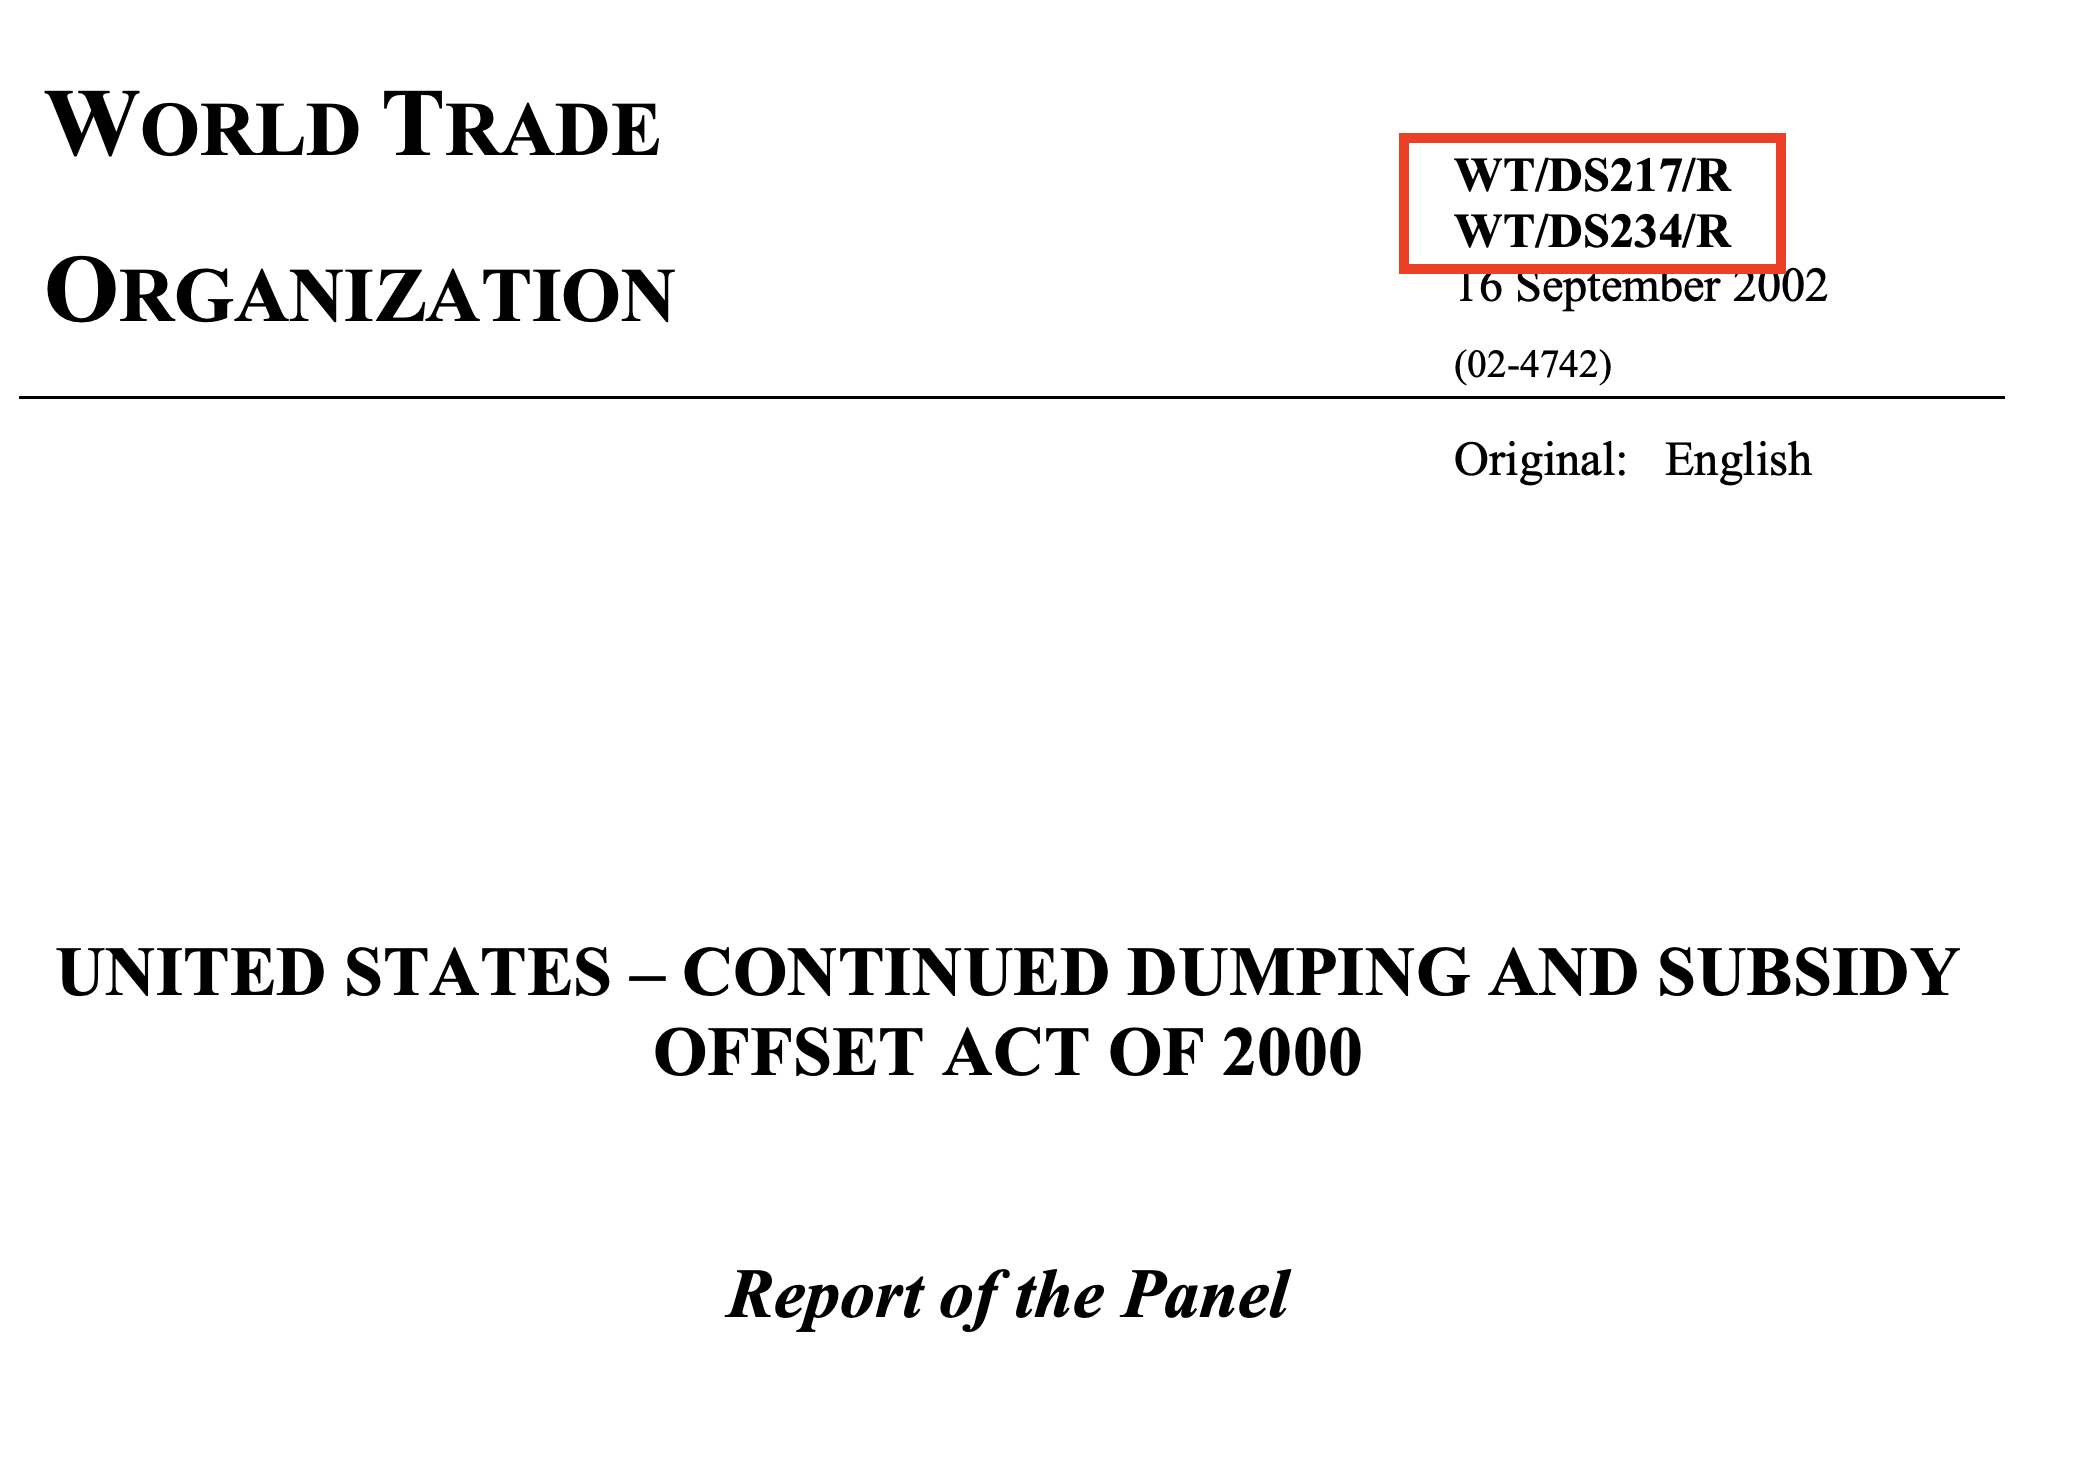
\includegraphics[scale=0.35]{Data/pngs/linked_cases.png}
    \caption{
        Panel explicitly marks which different cases are handled together in the cover of the panel report. DS217 and DS234 are handled togehter in this example.
        }
    \label{fig:linked-cases}
\end{figure}


% way before they express their
% legal conclusion as to the inconsistency  to the rules of the WTO or not.

% where the panel expresses 
% its conclusion as to whether the challenged 
% trade policy is inconsistent to the rules of the WTO or not.